\documentclass{article}

\usepackage[letterpaper]{geometry}
\usepackage{authblk}
\usepackage{graphicx}

% Prepend "S" on numbered items
\renewcommand{\thesection}{S\arabic{section}}
\renewcommand{\thefigure}{S\arabic{figure}}


% ---------------------------------------------------------------------------------------
% BEGIN TITLE AND AUTHORS
% ---------------------------------------------------------------------------------------
\title{Supplementary Material}

\author[a]{Colin T. Sullender}
\author[a]{Adam Santorelli}
\author[a]{Lisa M. Richards}
\author[a]{Pawan K. Mannava}
\author[a]{Christopher Smith}
\author[a,*]{Andrew K. Dunn}
\affil[a]{Department of Biomedical Engineering, The University of Texas at Austin, Austin, TX, 78712, USA}

\date{}


% ----------------------------------------------------------------------------------------
% BEGIN DOCUMENT
% ----------------------------------------------------------------------------------------
\begin{document}
\maketitle

\section{Importance of submerging the microfluidic outlet line}

One important experimental detail that all previous plots took into account was recording the flow profiles while the outlet tubing from the phantom was submerged in solution, as shown in Figs. 2 and 3. This was performed after visualizing the dramatic decrease in flow observed when the outlet line was elevated and the solution dripped into the outlet vial. The release of the drop from the end of the tubing caused a large decrease in pressure, resulting in a flow decrease. This was observed with both flow control systems as shown in Fig.~\ref{fig:supplement_outlet}, meaning that it is an important experimental consideration for any microfluidic setup. These trials included approximately five-minute duration with the outlet line elevated and allowed to drip into the outlet vial, followed by submersion of the outlet line in the solution for another five minutes. Thus, the large spike in relative flow corresponds to the time point where the outlet line was manually submerged in solution.

% Figure S1 - Outlet Line Submersion
\begin{figure}
    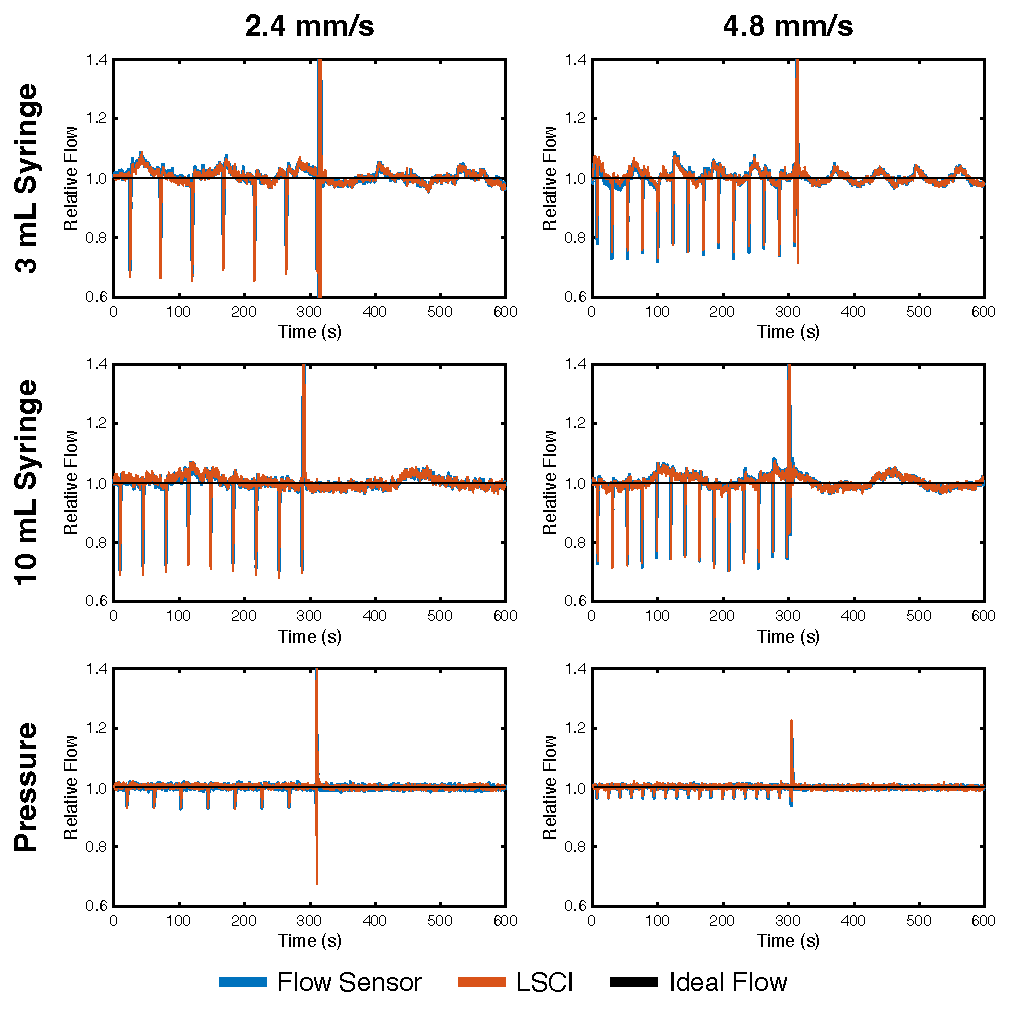
\includegraphics[width=\textwidth]{FigureS1.pdf}
    \caption {
        Impact of submerging the microfluidic device outlet tubing for both flow control systems at 2.4 and 4.8 mm/s as measured with the inline flow sensor (blue) and single-exposure LSCI (red). These trials show approximately five minutes of effluent dripping into the collection vial, as evidenced by the rapid periodic flow drops, followed by approximately five minutes of operation with the outlet tubing submerged in solution. All measurements were normalized to the average flow during the submerged segment of each experiment and compared to the ideal flow (black).
    }
    \label{fig:supplement_outlet}
\end{figure}

Some general trends were observed from these trials. First, the magnitude of the flow decrease was larger for the syringe pump versus the pressure system. Because the pressure system has a higher compliance than the syringe pump, high frequency perturbations are dampened more by the pressure system. The frequency of the droplets was also very regular within trials. This suggests that the drop must reach a similar critical volume regardless of flow rate to overcome the surface tension required to release the drop from the tubing. The mean volume of the droplets can be estimated using the absolute flow rate from the flow sensor and the time between drops, and a standard deviation of <0.5 µL in drop volume was observed within each trial. The magnitude of the flow decrease was also larger for the slower flow (2.4 mm/s) versus the faster flow (4.8 mm/s) for all trials. This is likely due to the larger pressure differential generated at slower flows, since the pressure driving the flow is smaller for the slower speed. For the pressure system, the drops led to a 1.4 mbar change in pressure for the 2.4 mm/s speed (28.3 mbar average), and a 1.1 mbar change in pressure for the 4.8 mm/s speed (47.4 mbar average). A larger pressure change for a lower average pressure produces to a larger change in flow, which agrees with the larger magnitude flow drop seen for the slower speeds. Overall, these plots demonstrate that the user should be aware of the position of the outlet line during microfluidic data acquisition, and that submersion of the outlet line is critical to eliminate rapid flow changes caused by dripping from the outlet line.


% ----------------------------------------------------------------------------------------
% END
% ----------------------------------------------------------------------------------------
\end{document}
